%!TEX root = ../final-report.tex
\chapter{Results}
\label{ch:results}

This chapter presents results for the four solvers. For each of the five initial conditions, the solvers will be compared for a few representative bathymetries. Reference results were obtained using the unbalanced solver from Section~\ref{sec:roe} on a very fine grid of 10,000 cells. At the end, the execution time of the different solvers is compared as well.

\section{Still Water}



\begin{figure}
  \centering
  \begin{subfigure}{\textwidth}
    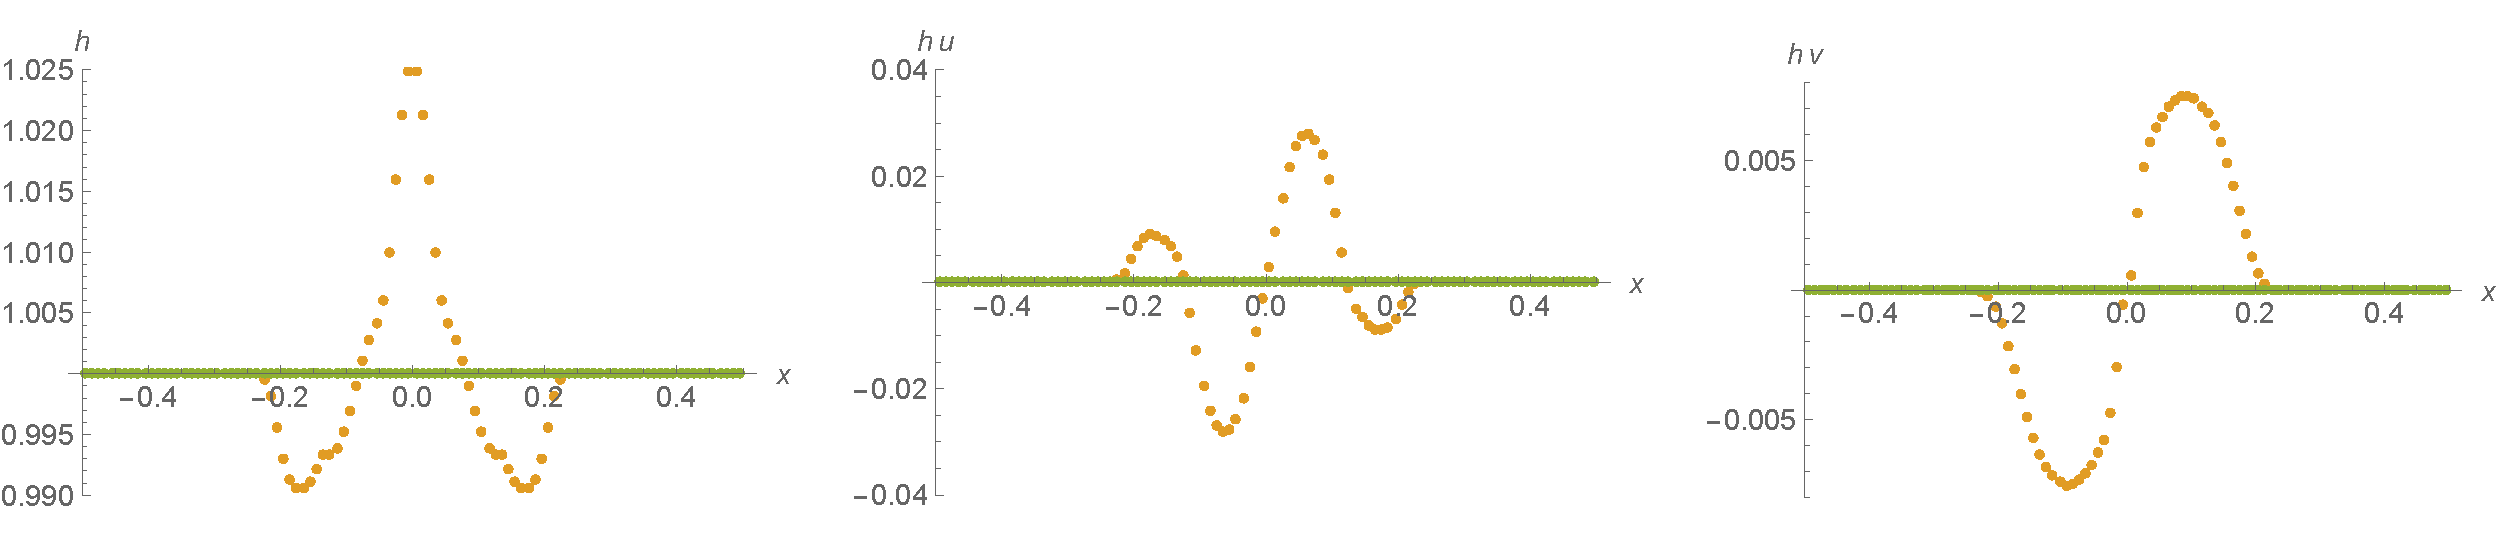
\includegraphics[width=\textwidth]{diagrams/results-still-1}
    \caption{$t = 0.1$}
    \label{fig:results-still-1}
  \end{subfigure} \\
  \begin{subfigure}{\textwidth}
    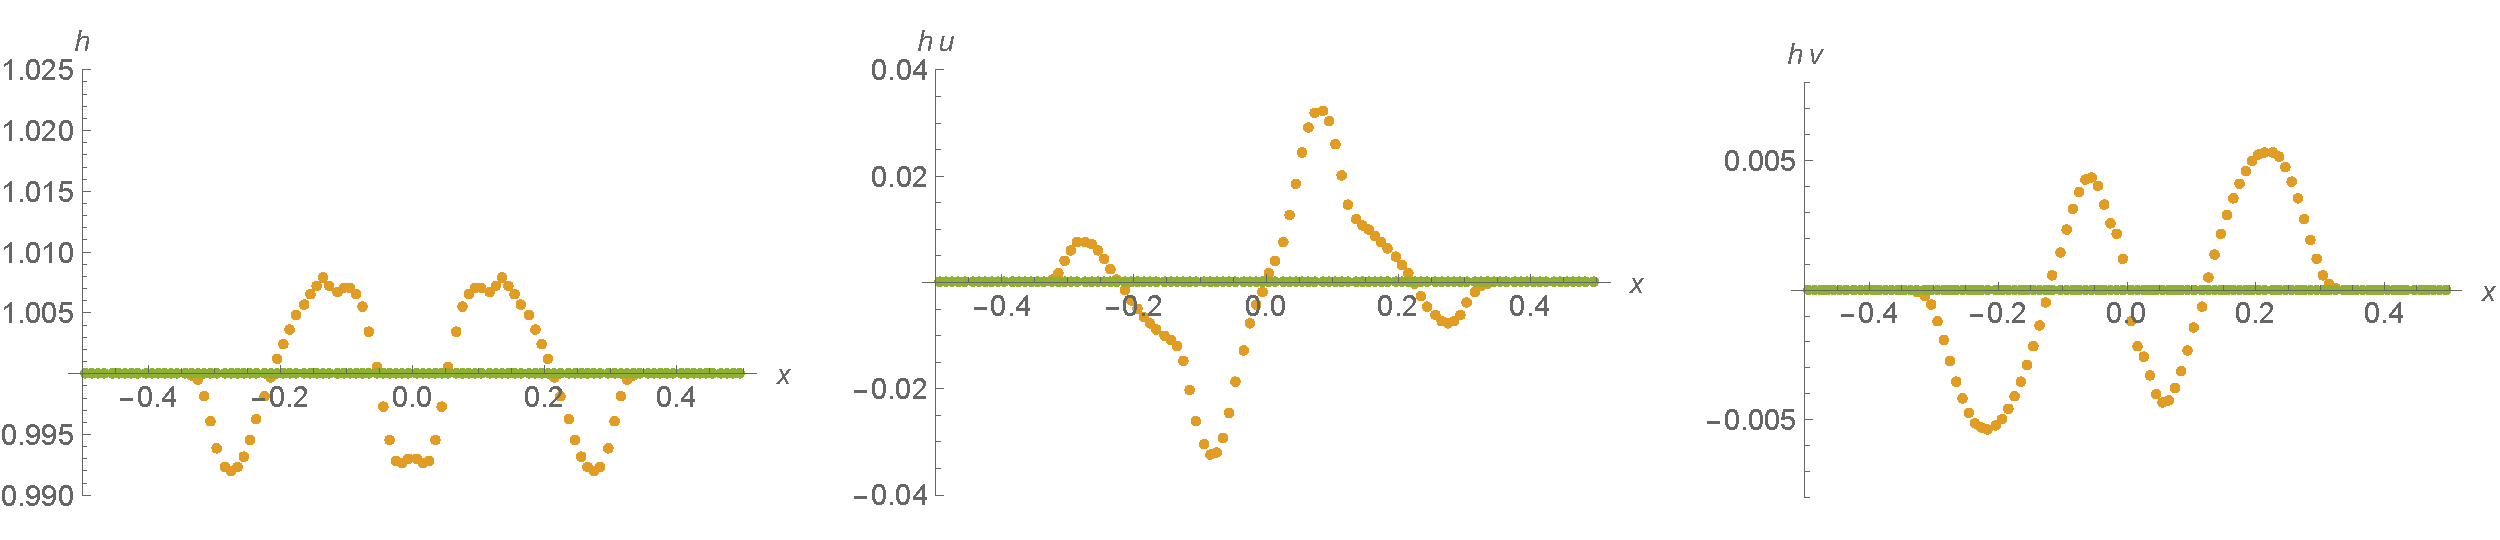
\includegraphics[width=\textwidth]{diagrams/results-still-2}
    \caption{$t = 0.2$}
    \label{fig:results-still-2}
  \end{subfigure} \\
  \begin{subfigure}{\textwidth}
    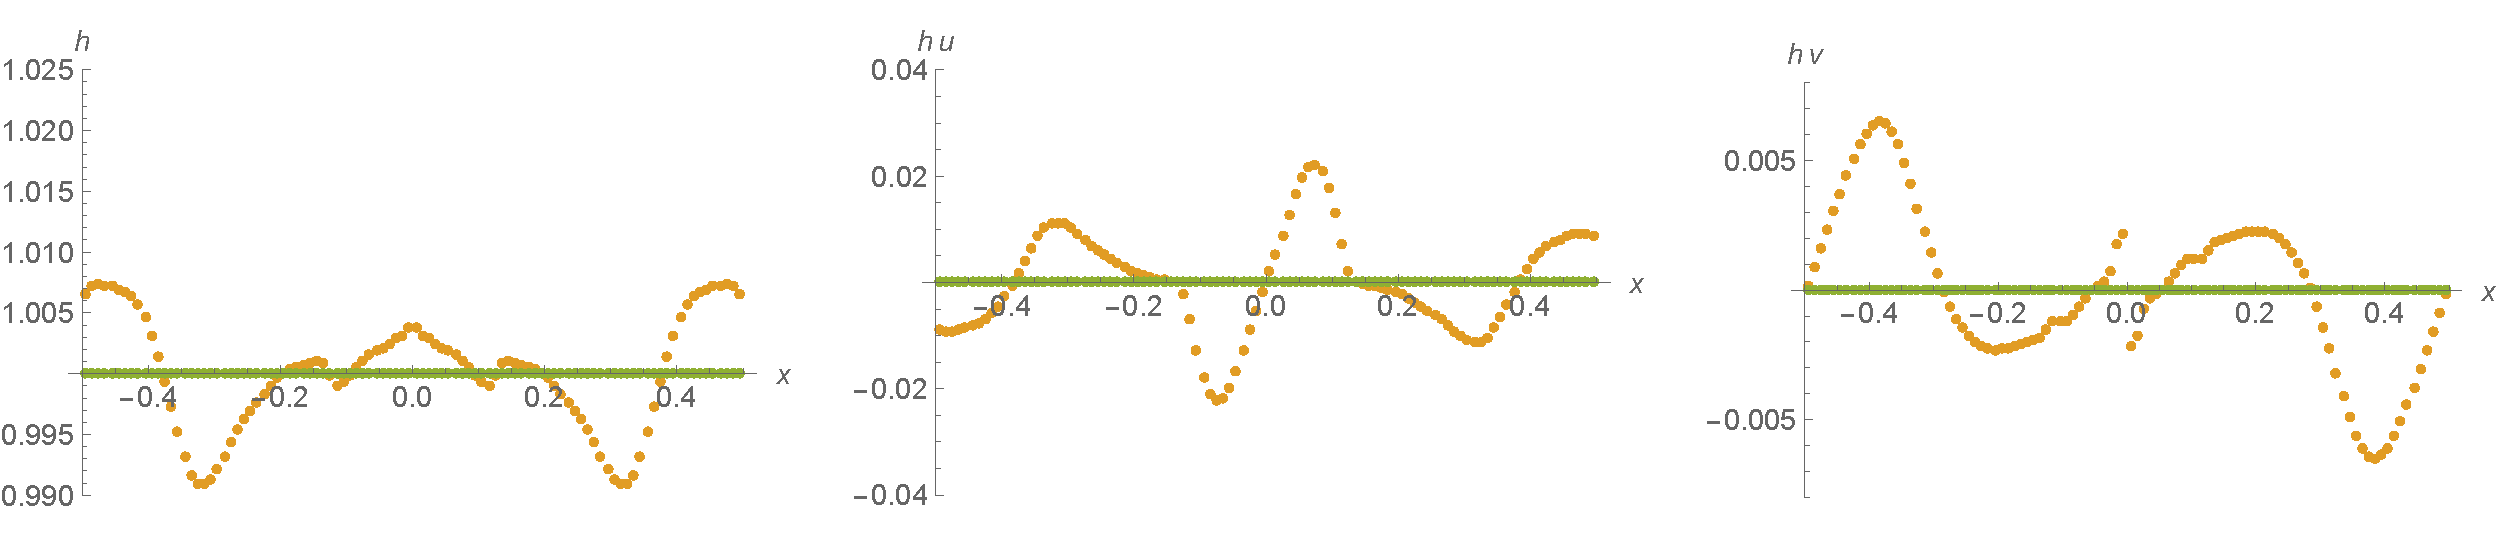
\includegraphics[width=\textwidth]{diagrams/results-still-5}
    \caption{$t = 0.5$}
    \label{fig:results-still-5}
  \end{subfigure} \\
  \begin{subfigure}{\textwidth}
    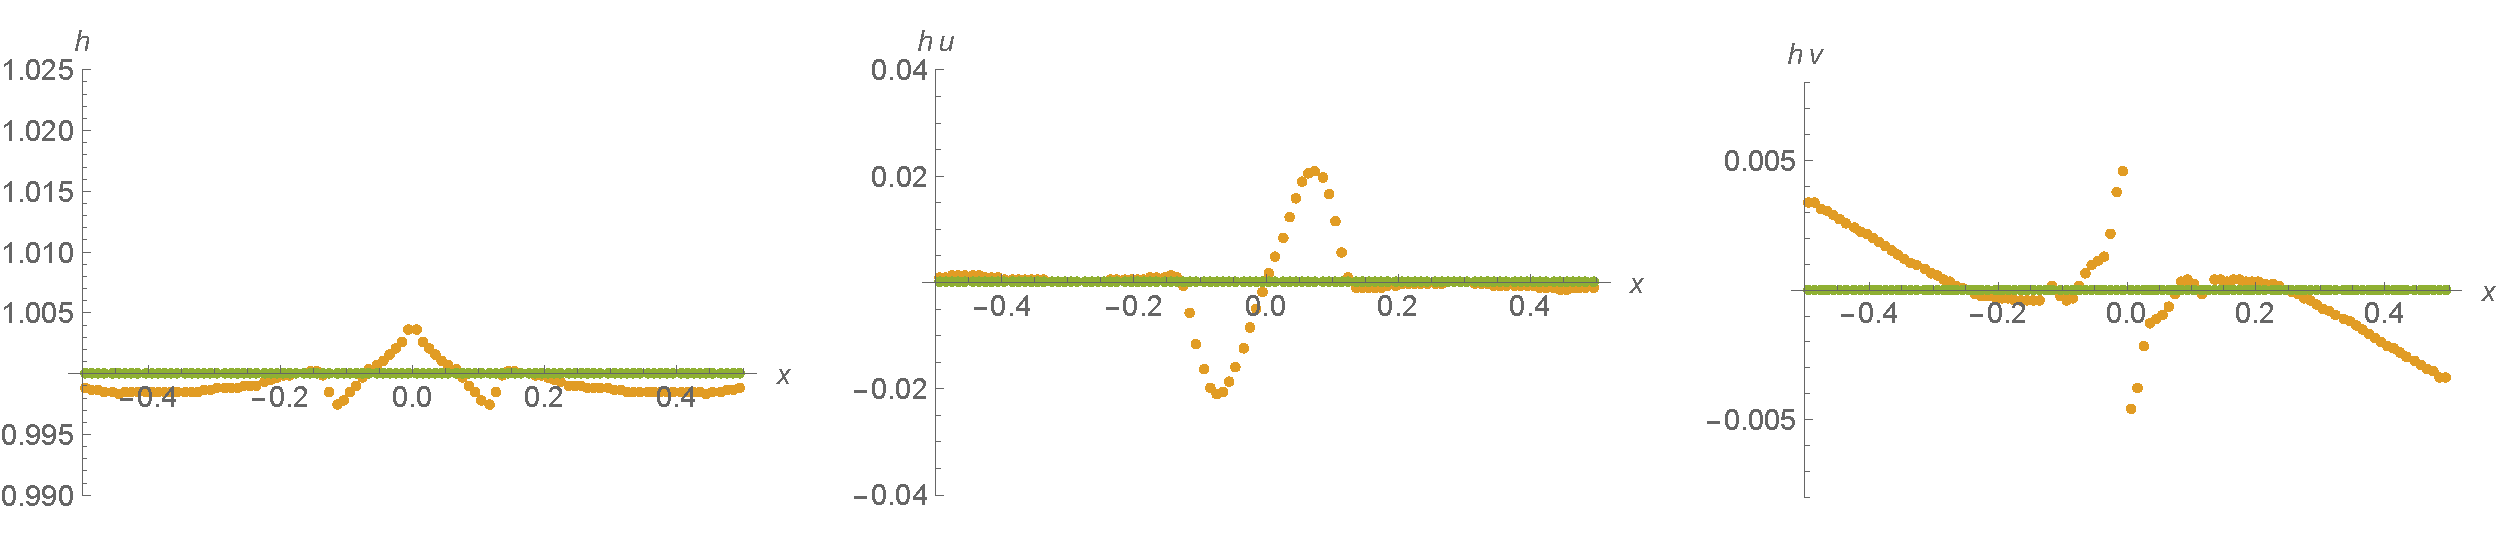
\includegraphics[width=\textwidth]{diagrams/results-still-10}
    \caption{$t = 1.0$}
    \label{fig:results-still-10}
  \end{subfigure}
  \caption{Results for still water over a cosine ridge. The exact solution is $h = 1$, $hu = hv = 0$ for all times. The orange data was obtained with the unbalanced solver over 100 grid cells.  The green data corresponds to any of the three balanced solvers.}
  \label{fig:results-still}
\end{figure}

\section{Wave through Still Water}

\section{Geostrophic Equilibrium}

\section{Wave through Geostrophic Equilibrium}

\section{Uniform Flow}

\section{Execution Time}

\begin{itemize}
  \item show how unbalanced method fails
  \item go through different methods, showing where they work and where they fail
\end{itemize}